\begin{figure}[b]
%  \centering
   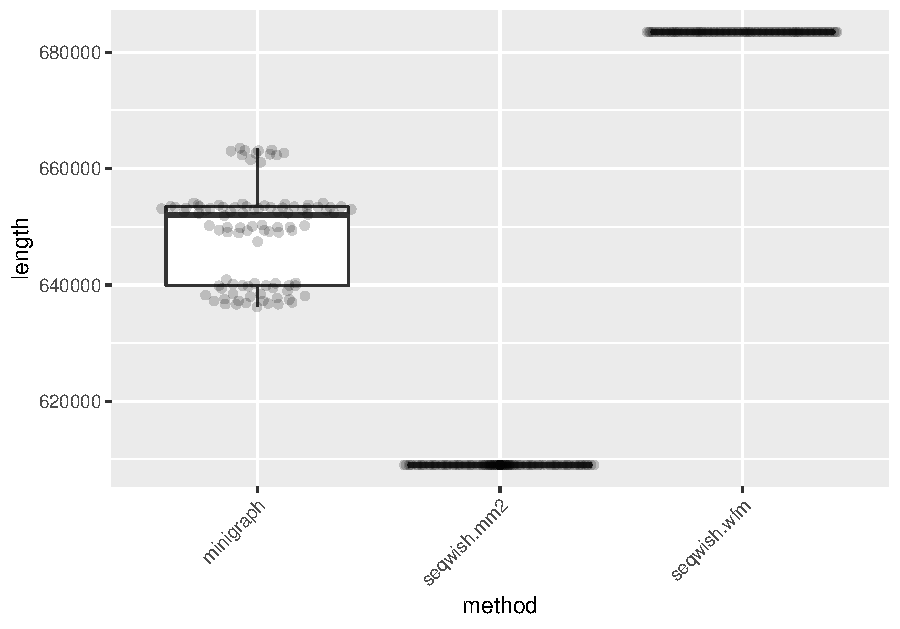
\includegraphics[width=\linewidth]{yeast_chrV_length_vs_100orders}
   \caption{
     Base-pair lengths of graphs built from 100 permutations of yeast chrV.
     Each point corresponds to the length of a graph built from a specific permutation and the given method.
     We color each point by the first genome in the order (the ``reference'' in \textit{minigraph}).
     A boxplot per first genome group provides the mean and the first and third quartile intervals for each reference grouping.
    }
    \label{fig:yeast}
\end{figure}
